\documentclass[letterpaper,12pt]{article}
\usepackage[margin=1in]{geometry}
\usepackage{graphicx}  % Include figure files
\usepackage{xcolor}  % Allow for a color text
\usepackage{amsmath}  % math fonts
\usepackage{amsfonts}  % math fonts
\usepackage{latexsym}  % math fonts
\usepackage{amssymb}  % math fonts
\usepackage{mathtools} % Give more control of how equations are displayed
\usepackage{appendix} % Lets you create an appendix
\usepackage[numbered]{matlab-prettifier} % Let's me import MATLAB code in a nice format
\usepackage{indentfirst} % This indents the first paragraph. By default latex won't do it.

\setlength{\parskip}{1em} % This skips a line when making new paragraphs
\newtagform{show_eq}{(Eq.\ }{)}  % how the equation numbers are displayed
\usetagform{show_eq} % this goes with the \newtagform

\begin{document}

% ================================== Title Page ==========================================
\begin{titlepage}
 \begin{center}
 \vspace*{1in}
{\Huge Examination of LM741 Operational Amplifier in High and Low Gain Configurations}\\
    \bigskip
    by\\
    \bigskip
    {\Large Kevin Moran} \\
    \bigskip
    Lab Partner : Jorge Soberanis\\
    Date of Experiment : Thursday, October 14th, 2020

    \bigskip\bigskip\bigskip
    University of Southern California\\
    Aerospace and Mechanical Engineering Department\\
    AME 341A : Mechoptronics
 \end{center}
\end{titlepage}


% ================================== Main Text =====================================


% --------------------------------- Introduction -----------------------------------
\section{Introduction}
Operational Amplifiers, often referred to as \textit{op-amps}, are a vital part of data acquisition circuits and circuits that rely on threshold voltage inputs to activate additional components. As the name suggest, op-amps serve as voltage amplifiers and can be setup in various configurations using passive circuit elements such as resistors and capacitors. Figure \ref{NFL} illustrates a LM741 op-amp in a negative feedback loop configuration.

\begin{figure}[ht]
    \centering
    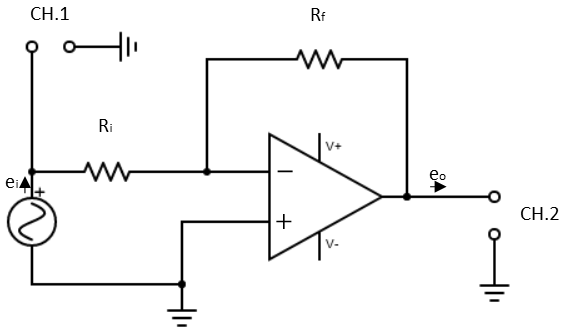
\includegraphics[scale=1.25]{feedback.png}
    \caption{\small LM741 operational amplifier negative feedback loop schematic. All components of the circuit are grounded using a common ground. CH1 and CH2 represent probe connection on the Vbench Interface.}
    \label{NFL}
\end{figure}
% ~~~~~~~~~~~~~~~~~~~~~~~~~~~~~~~ Gain ~~~~~~~~~~~~~~~~~~~~~~~~~~~~~~~~~~~~~~~~~~~~
\subsection{Gain}
In an open loop configuration, the output voltage of an op-amp quickly reaches saturation and may not provide useful results in many data acquisition applications. A negative feedback loop, however, allows for greater control over amplification characteristics. Referred to as \textit{gain}, the relationship between input and output voltages can be expressed as :

\begin{equation}
    \label{Gain}
    e_o = -Ge_i = -\frac{R_f}{R_i}e_i
\end{equation}
$G$ represents gain, and $R_f$ and $R_i$ correspond to resistors shown in Figure \ref{NFL}. The negative sign in Equation \ref{Gain} is a consequence of the input voltage, $e_i$, feeding into the inverting channel on the op-amp, and $e_o$ represents the output voltage from the op-amp. Unlike passive circuit elements, op-amps need an external power source to operate. The power supply is shown by the inputs V+ and V-.

% ~~~~~~~~~~~~~~~~~~~~~~~~~~~~~~~ 1st Order Sys ~~~~~~~~~~~~~~~~~~~~~~~~~~~~~~~~~~
\subsection{First Order System}
Developing a first order differential equation and making the assumption $R_f >> R_i$ yields 
\begin{equation}
    \label{1stOrder}
    \frac{\mu R_f}{A R_i}\frac{de_o}{dt} + e_o = -\frac{R_f}{R_i}e_i 
\end{equation}
where variables $\mu$ and $A$ are properties of a given op-amp. Solving the first order ODE yields a complex solution, however, deriving a transfer function and taking the modulus produces a semi-theoretical model : 
\begin{equation}
    \label{Htheo}
    |H|_{theo} = \frac{R_f/R_i}{\sqrt{1 + \omega^2(\frac{\mu}{A}\frac{R_f}{R_i})^2}}
\end{equation}
Since $\mu$ and $A$ are experimentally derive quantities, the subscript \textit{theo} denotes a semi-theoretical model, and the natural frequency, $\omega$, can be rewritten in terms of frequency as $\omega = 2\pi f$. Furthermore, the modulus of the transfer function can also be written in terms of input and output voltage as
\begin{equation}
    \label{Hexp}
    |H|_{exp} = \frac{e_o}{e_i}
\end{equation}
where the subscript \textit{exp} refers to a model that is exclusively dependent on variables measured during the experiment.

% ~~~~~~~~~~~~~~~~~~~~~~~~~~~~~~~ f0 and GBP ~~~~~~~~~~~~~~~~~~~~~~~~~~~~~~~~~~~~~~
\subsection{Cutoff Frequency and Gain Bandwidth Product}
In a negative feedback loop, the relationship between amplification and frequency can be categorized by three distinct regions :
\begin{align*}
    2 \pi f \frac{\mu R_f}{A R_i} << 1 &  \Rightarrow |H| = G \\
    2 \pi f \frac{\mu R_f}{A R_i} >> 1 &  \Rightarrow |H| = 1 \\
    2 \pi f \frac{\mu R_f}{A R_i} \ =1 &  \Rightarrow |H| = \frac{G}{\sqrt{2}}
\end{align*}
The latter of the regions represents a particularly interesting relationship known as a circuits cutoff frequency. Explicitly defined by the relationship,
\begin{equation}
    \label{cutoff}
    f_0 = \frac{A R_i}{2\pi \mu R_f}
\end{equation}
the cutoff frequency, $f_0$, is the frequency at which the circuit can no longer effectively amplify the input voltage and thus, begins to attenuate the signal. In addition to identifying the range of frequencies for optimal gain in a given circuit, the cutoff frequency is also important for defining an op-amps Gain Bandwidth Product (GBP). Represented by the variable $f^*$ in Equation 6, GBP is strictly a property of the op-amp in the circuit. This governs the inverse relationship between gain and cutoff frequency (i.e., as gain increases, cutoff frequency decreases and vice versa).
\begin{equation}
    \label{GBP}
    f^* = f_0G
\end{equation}

\begin{figure}[ht]
    \centering
    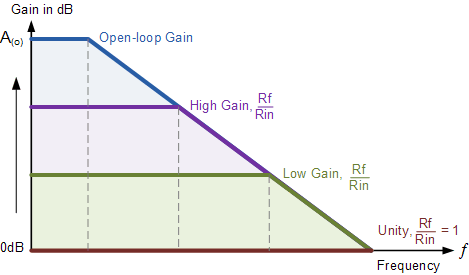
\includegraphics[scale = .5]{GBPpic.png}
    \label{GBPpic}
    \caption{\small The relationship between cutoff frequency (vertical dashed lines) and gain (horizontal lines), for a given op-amp. Lowering the gain of a circuit allows for a greater frequency range. Image courtesy of \textit{electronics-tutorials.ws}}
\end{figure}


% -------------------------- Methods and Materials ------------------------------
\section{Procedures}
\subsection{Materials and Experiment Setup}
By using a National Instruments VirtualBench VB-8012 to take measurements and control input signals, the LM741 op-amp was characterized using frequencies ranging from 100Hz to 1MHz. The experiment consisted of two nearly identical circuits with subtle differences in input resistors. Input resistors were selected based on nominal values of 20k$\Omega$ and 2k$\Omega$ for setups 1 and 2, respectively. The feedback resistor was selected based on a nominal value of 200k$\Omega$ and was kept throughout the entire experiment. This selection of resistors ensured setup 1 and setup 2 resulted in low and high gain circuits, respectively. All resistors were measured before being integrated into the circuit. Channel 1 and channel 2 were setup to measure input and output voltages, and all grounds were connected to a common ground. Both experimental setups were based on the schematic shown in Figure \ref{NFL} and followed identical procedures. 

\subsection{Methods}
Beginning with a frequency of 100Hz, the experimental gain was calculated by taking the ratio between measured values of output and input voltages. According to the semi-theoretical model, the ratio between output and input voltages should be equal to the ratio between feedback and input resistors. This served as the initial benchmark for comparing the experimental and semi-theoretical models.

Since it was known that the relationship between gain and frequency is non-linear near the cutoff frequency, input and output voltage measurements were concentrated in this region. Initial guesses for the cutoff frequency were determined by estimating what the output voltage would need to be to satisfy the requirement $e_o/e_i = G/\sqrt{2}$. Since $e_i$ was relatively constant, the frequency was adjusted in a series of trial and error modifications until $e_o$ was measured within the appropriate value. Once the cutoff frequency was determined within reasonable experimental expectation, input and output voltages were measured, used to calculate amplification via Equation \ref{Hexp}, and plotted on a log-log scale until the non-linear region of the $|H|\ vs\ f$ graph was well characterized. Afterwards, the linear regions were characterized by taking a enough data to adequately represent the system response to relatively high and low frequencies. Approximately five to ten data points in each linear region were obtained, ensuring the frequency values were spaced out evenly to cover the entire region.

% --------------------------------- Results ---------------------------------------
\section{Results}
Gain as a function of input frequency for the low gain negative feedback circuit is plotted in Figure \ref{LowG}. Additionally, the semi-theoretical model expressed in Equation \ref{Htheo} is also plotted for comparison between experimental and anticipated results.  

\begin{figure}[ht]
    \centering
    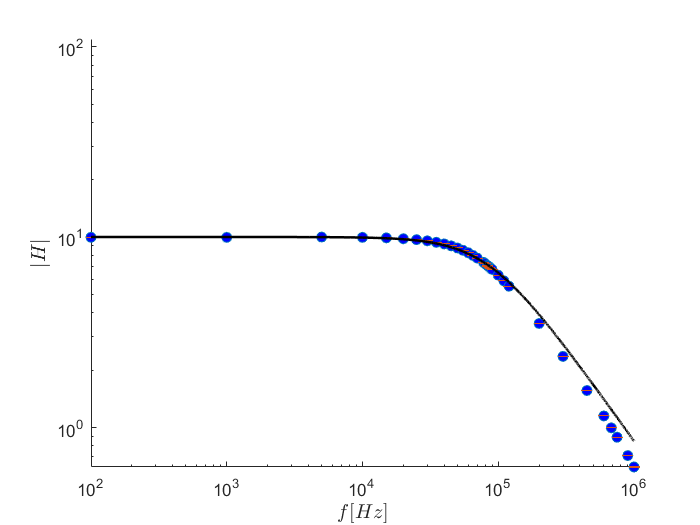
\includegraphics[scale = .6]{LowGain.png}
    \caption{Setup 1 with op-amp in a low gain configuration}
    \label{LowG}
\end{figure}
It is clear that semi-theoretical and experimental models expressed in Equations \ref{Htheo} and \ref{Hexp} are in agreement until the system approaches the cutoff frequency. Beyond the cutoff frequency, however, the two models begin to diverge and the experimental data shows a lower than anticipated gain.

Figure \ref{HighG} shows gain versus input frequency data for the high gain negative feedback circuit. In this configuration, the experimental and semi-theoretical models agree throughout the entire domain of frequencies tested.

\begin{figure}[ht]
    \centering
    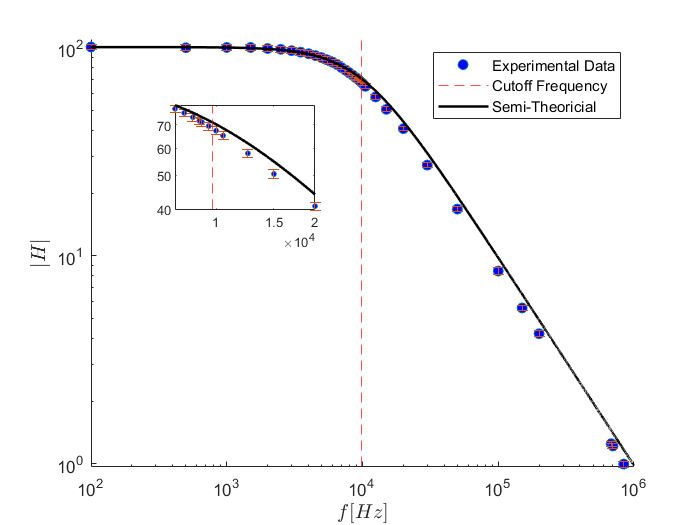
\includegraphics[scale = .6]{HighGain.png}
    \caption{Setup 2 with op-amp in a high gain configuration}
    \label{HighG}
\end{figure}
As anticipated, the cutoff frequency was significantly reduced as a consequence of the greater amount of gain generated. Both experimental sets of data also support the GBP as a property of the op-amp rather then other circuit elements. Regardless of the resistors chosen to create the circuit, both high and low gain configurations converged towards the same GBP. Thus, both circuits have a unique usable range for amplification that matches the ideal gain expressed in Equation \ref{Gain}. In either case, the usable range can be defined by the relationship $f<<f_0$, that is, the horizontal regions in Figures \ref{LowG} and \ref{HighG}.

\subsection{Experimental Error}
To conclud whether experimental and theoretical gain are equivalent, the associated error of each quantity must be taken into account. Furthermore, since experimental gain changes as the system approaches cutoff frequency, the analysis shall be performed using a low frequency data point (i.e., 100Hz). Equations \ref{dGexp} and \ref{dGtheo} represent the relative uncertainties for experimental and theoretical gain. 

\begin{equation}
    \Delta G_{exp} = G_{exp} \sqrt{ (\frac{\Delta e_i}{e_i})^2 + (\frac{\Delta e_0}{e_0})^2}
    \label{dGexp}
\end{equation}
\begin{equation}
    \Delta G_{theo} = G_{theo}\sqrt{(\frac{\Delta R_i}{R_i})^2 + (\frac{\Delta R_0}{R_0})^2 }
    \label{dGtheo}
\end{equation}

Since the cutoff frequency in each setup consisted of scanning through various frequencies until the amplification fell within the appropriate window, the cutoff frequency and its uncertainty can be expressed using the following set of equations,
\begin{equation}
    \begin{split}
        f_0 = \frac{f_{high} + f_{low}}{2}\\
        \Delta f_0 = \frac{f_{high} - f_{low}}{2}
    \end{split}
\end{equation}
where the subscripts \textit{high} and \textit{low} denote the two frequencies used to fulfill the amplification requirement.

Table \ref{KeyValues} summarizes key values, as well as respective uncertainties. It is shown that $G_{exp} \pm{\Delta G_{exp}} = G_{theo} \pm{\Delta G_{theo}}$ in both low and high gain configurations.
\begin{table}[ht]
    \centering
    \begin{tabular}{ c | c | c | c ||c | c | c | c }
    \multicolumn{8}{c}{Key Values} \\
    \hline
    $R_f$ & 196960 & $\Delta R_f$ & 1970 & $e_{i,1}$ & .097 & $\Delta e_{i,1}$ & .002  \\
    $R_{i,1}$ & 19649 & $\Delta R_{i,1}$ & 197 & $e_{o,1}$ & .973 & $\Delta e_{o,1}$ & .016    \\
    $R_{i,2}$ & 1958 & $\Delta R_{i,2}$ & 20 & $e_{i,2}$ & .068 & $\Delta e_{i,2}$ & .002     \\
    $f_{0,1}$ & 85000 & $\Delta f_{0,1}$ & 1000 & $e_{o,2}$ & 6.88 & $\Delta e_{o,2}$ & .156  \\
    $f_{0,2}$ & 9750 & $\Delta f_{0,2}$ & 250 &  $f^*$ & $9.8*10^{5}$ & $\Delta f^*$ & 28720  \\
    \hline
    $G_{exp,1}$ & 10 & $\Delta G_{exp,1}$ & .2 & $G_{theo,1}$ & 10 & $\Delta G_{theo,1}$ & .1 \\
    $G_{exp,2}$ & 101 & $\Delta G_{exp,2}$ & 3.2 & $G_{theo,2}$ & 101 & $\Delta G_{theo,2}$ & 1.4 
    \end{tabular}
    \caption{\small Subscripts 1 and 2 denote experiment setups 1 and 2. Additionally, the subscripts i,o,and f denote input, output and feedback,respectively. For convenience, the uncertainty of each resistor was taken to be $\pm{1\%}$.}
    \label{KeyValues}
\end{table}

% --------------------------------- MATLAB ----------------------------------------
\newpage
\appendix
\section{MATLAB Script}
\lstinputlisting[style=Matlab-editor]{lab6.m}

\end{document}